% Anonymized working manuscript for FISAT 2026.
% Keep \anonymoustrue for review. Replace every camera-ready placeholder only
% after all authors have verified it. Numerical results are never typed here:
% scripts/analyze_results.py generates the files conditionally included below.
\documentclass[runningheads]{llncs}

\usepackage{amsmath}
\usepackage{amssymb}
\usepackage{booktabs}
\usepackage{graphicx}
\usepackage{url}

% Springer production can extract these descriptions even when the local class
% does not typeset them. The same text is also exported to figures/alt-text.txt.
\providecommand{\Description}[1]{}

\newif\ifanonymous
\anonymoustrue

\newcommand{\pendingresults}[1]{%
  \begin{center}
    \fbox{\parbox{0.92\linewidth}{\textbf{RESULTS PENDING:} #1}}
  \end{center}}
\newcommand{\artifactlocation}{[ANONYMIZED ARTIFACT URL/DOI REQUIRED]}
\newcommand{\intereststatement}{[AUTHOR-CONFIRMED DISCLOSURE REQUIRED]}

\begin{document}

\title{Missing Is Not Normal: Quality-Aware Microservice Root-Cause
Ranking under Structured Telemetry Loss}
\titlerunning{Quality-Aware RCA under Structured Telemetry Loss}

\ifanonymous
  \author{Anonymous Author(s)}
  \authorrunning{Anonymous Author(s)}
  \institute{Anonymous Institution(s)}
\else
  % Camera-ready metadata: replace only after every author confirms the order,
  % affiliation, email, ORCID, and corresponding-author designation.
  \author{Nguyen Quoc Bao Huy\inst{1}\orcidID{0009-0001-7091-2406}}
  \authorrunning{N. Q. B. Huy}
  \institute{FPT University, Ho Chi Minh City, Vietnam\\
  \email{nqbhuy2004nt@gmail.com}}
\fi

\maketitle

\begin{abstract}
Microservice root-cause analysis (RCA) is commonly evaluated as though all
telemetry streams remain available throughout an incident. That assumption is
fragile: sampling, backpressure, exporter failure, and network partitions can
remove precisely the evidence needed for diagnosis. We study service-level
localization under four reproducible forms of metric loss: isolated missing
points, channel-local bursts, complete stream loss, and incident-correlated loss
that preferentially hides large deviations. We introduce QARCA, a
quality-aware logistic ranker that combines distribution-shift evidence with
availability, gap, continuity, and cross-service features without using service
or system identities. Evaluation uses all 375 metric incidents in RCAEval RE1,
three leave-one-system-out folds, three loss rates, and ten matched masks per
condition. Comparators are N-Sigma, BARO, and a robust median-shift baseline;
the primary endpoint is service-level mean reciprocal rank, with per-incident
paired inference and robustness area under the loss-rate curve. Training masks
are isolated from test masks, and all numerical claims are generated from saved
per-incident predictions. This design separates localization from incident
detection by supplying the injection boundary and explicitly reports cases in
which root-service evidence is absent.
\IfFileExists{generated/abstract_result.tex}{%
  % Generated; do not edit.
Across 375 RCAEval incidents and four synthetic metric-loss mechanisms up to 50\%, QARCA achieved mean per-incident MRR AUC 0.857, compared with 0.653 for the strongest evaluated baseline.
%
}{%
  \textbf{This working manuscript does not assert numerical outcomes until the
  frozen experiment has completed.}%
}

\keywords{Microservices \and Root-cause analysis \and Missing telemetry
\and Observability \and Robust ranking}
\end{abstract}

\section{Introduction}

Microservices make independent deployment and scaling possible, but they also
spread one user-visible failure over services, hosts, queues, and network
links. Operators therefore depend on metrics, logs, and traces to localize an
incident. In production, however, observability is a resource-constrained
distributed system in its own right. Traces are sampled, exporters and
collectors can fall behind, and best-effort transport loses data
\cite{observability2022,canopy2017,telemetryloss2018}. A diagnostic method can
then face two simultaneous changes: the system's behavior changes, and the
record of that behavior becomes incomplete.

Many RCA evaluations leave this second change implicit. Complete benchmark
windows make methods easy to compare, but they cannot reveal whether a ranking
is robust to an isolated gap, a collector outage, a failed metric channel, or
preferential loss around the most anomalous portion of an incident. Treating
all missingness as independent random deletion is also inadequate. A burst can
erase temporal continuity while preserving the same overall number of cells as
uniform loss; whole-stream loss can remove every metric belonging to the true
service; and overload-related loss can be statistically coupled to the failure
being diagnosed.

Recent work has begun to address incomplete or unreliable telemetry
\cite{reconrca2025,latentscope2024,mhprca2026} and call-graph blind spots or
lightweight robust diagnosis \cite{torai2026,fukuda2025robust}.
Our claim is deliberately narrower than being the first study of missing-data
RCA. We contribute a controlled, matched evaluation of several structured loss
mechanisms on a public benchmark, together with a small service ranker whose
inputs expose both anomaly strength and evidence quality. This boundary matters:
the study asks whether an explicitly quality-aware ranking rule generalizes to
an unseen microservice system, not whether one learned model subsumes every RCA
modality or production failure mode.

The paper makes three methodological contributions:

\begin{enumerate}
\item We define deterministic point, channel-local burst, whole-stream, and
incident-correlated corruptions at 10\%, 30\%, and 50\% nominal loss. All
methods receive matched masks, and the ten masks within an incident are treated
as repeated measurements rather than independent failures.
\item We introduce QARCA, a 114-feature service ranker that retains missingness
as evidence. It combines classical and robust distribution shifts with
coverage, gap, continuity, metric-kind, and relative cross-service summaries.
Training and evaluation follow leave-one-system-out (LOSO) separation; labels,
fault names, service identities, and system identities are excluded from model
features.
\item We freeze a reproducible analysis protocol around all 375 RCAEval RE1
incidents \cite{rcaeval2025}. It reports unconditional performance, performance
conditional on observable root evidence, robustness across loss rates, paired
uncertainty, ablations, and runtime. Per-incident predictions and analysis
tables are artifact outputs rather than manually transcribed values.
\end{enumerate}

The remainder distinguishes the benchmark's injected service label from a
unique socio-technical ``root cause.'' We evaluate localization of that label
given a known incident boundary. We do not evaluate anomaly detection, explain
human or organizational causes, or claim that synthetic deletion reproduces a
production telemetry outage.

\section{Background and Related Work}

\subsection{Microservice RCA and its evaluation}

Microservice RCA methods draw on different evidence and assumptions. Statistical
scorers rank unusual metric changes; BARO provides a robust metric-ranking
baseline and an associated N-Sigma comparator \cite{baro2024}. Trace-based
approaches exploit request execution and latency structure
\cite{microrank2021,tracerca2021,epsilonDiagnosis2019}. Other approaches infer
causal or conditional-dependence structure from telemetry, including
MicroCause, RCD, CIRCA, and later causal RCA variants
\cite{microcause2020,ikram2022rcd,circa2022,causalrca2023,pham2024causal}.
These methods are not interchangeable: some require a call graph, traces, or
multiple historical incidents, whereas a metric scorer can operate on one
window and a supplied boundary.

Benchmark choice can dominate conclusions. DeathStarBench established a broad
suite for studying microservice systems \cite{deathstarbench2019}; Train Ticket
supports software-engineering fault studies \cite{trainticket2021}; and the
PetShop dataset targets causes of performance issues \cite{petshop2024}.
RCAEval standardizes several RCA datasets and methods and makes per-failure
telemetry available \cite{rcaeval2025}. We use only its RE1 metric subset so
that every comparator receives the same modality and every incident has a
service-level injected label. Online Boutique and Sock Shop are additionally
cited through their maintained source repositories
\cite{googleOnlineBoutique,weaveworksSockShop}.

\subsection{Incomplete evidence is part of the diagnosis problem}

Missing telemetry is not one condition. Independent point loss approximately
models sampling or sporadic transport failures. A channel-local burst represents
a temporary interruption affecting one metric at a time, not a synchronized
collector-wide outage. Stream loss represents an exporter,
instrument, or routing failure that removes one metric channel throughout the
window. Incident-correlated loss is a stress case for missing-not-at-random
(MNAR) behavior: cells with larger incident-time deviations are more likely to
be absent. The last case is particularly important because a method that looks
robust under uniform deletion may still fail when observability degrades during
the anomalous interval.

Methods such as ReconRCA, LatentScope, MHP-RCA, TORAI, and other recent robust
RCA proposals explicitly consider incomplete, heterogeneous, or unreliable
telemetry \cite{reconrca2025,latentscope2024,mhprca2026,torai2026,%
fukuda2025robust}. Their data modalities, corruption assumptions, and output
targets differ, so we do not treat their reported numbers as directly
comparable to RE1 service ranking. Our empirical gap is instead a matched
stress test: hold the incident and deletion budget fixed, vary deletion
structure, and compare a quality-aware learned ranker against reproducible
metric baselines. This framing also avoids attributing all performance change
to an imputer, which can conceal whether a method had usable evidence.

\section{Problem Formulation and Research Questions}

Let a latent incident window be $X\in\mathbb{R}^{T\times d}$ with $d$ metric
streams, known boundary $\tau$, and candidate services $\mathcal{S}$. The
benchmark supplies an injected service $s^*\in\mathcal{S}$ and an original
availability mask $M_0$; cells absent in the archive are never reconstructed.
An added-loss mask $A$ produces observed input
$\widetilde{X}=(M_0\odot A)\odot X$, with unavailable cells represented as
missing rather than zero. A localizer assigns scores to the fixed universe
$\mathcal{S}$. For injected-service score $g_{s^*}$, its conservative tied rank
is $r=|\{s:g_s\geq g_{s^*}\}|$, and reciprocal rank is $1/r$.

The boundary $\tau$ is supplied to every method. Values before $\tau$ form the
reference period and values at or after it form the incident period. This
choice isolates localization from change-point detection and prevents one
method's detector from receiving an unintended advantage. Labels encoded in
folder names are read only by training-label construction and evaluation; the
corruptor and feature extractor do not receive the fault type.

We ask:

\begin{description}
\item[RQ1:] How do matched point, channel-local burst, whole-stream, and
incident-correlated loss change service-level localization as loss increases?
\item[RQ2:] Does QARCA improve robustness over N-Sigma, BARO, and robust
median shift when the entire test system is unseen during training?
\item[RQ3:] Which mechanisms and fault groups produce observational ambiguity,
particularly when evidence from the injected service is partly or wholly
absent, and what confidence signals could support abstention?
\item[RQ4:] What changes when quality features or corruption augmentation are
removed, and what runtime cost accompanies the learned ranker?
\end{description}

\section{Quality-Aware Root-Cause Ranking}

\subsection{Metric evidence without backward leakage}

QARCA extracts each metric independently before pooling evidence by service.
For metric $j$, let $B_j$ and $A_j$ denote the finite observations before and
after $\tau$. Classical reference location and scale are the pre-incident mean
and standard deviation. Robust location is the median; robust scale is the
maximum of scaled median absolute deviation, scaled interquartile range, and a
small magnitude-dependent floor \cite{rousseeuw1993}. Post-incident samples are never used to
estimate a pre-incident reference.

Six nonnegative anomaly summaries are computed: maximum standardized
deviation, maximum robust deviation, classical and robust median shifts, and
the mean and maximum robust displacement of quantiles
$q\in\{.10,.25,.50,.75,.90\}$. Effects are clipped at $10^6$ and transformed
by $\log(1+|\cdot|)$. When a reference or post-incident sample is unavailable,
the anomaly value is zero while explicit validity and availability features
record why it is zero. Thus ``no measured deviation'' is distinguishable from
``no evidence.''

For comparators that cannot accept missing values, preprocessing is causal in
time: forward fill is followed by a median computed only from the pre-incident
window; a wholly absent stream becomes constant zero and is subsequently
uninformative. No post-incident value is carried backward into the reference
period.

\subsection{Quality and service-level feature schema}

Table~\ref{tab:features} gives the fixed 114-dimensional schema. Metric-level
quality summaries include pre- and post-availability, their harmonic mean,
longest missing gaps normalized by period length, coverage over ten contiguous
post-incident blocks, fraction and longest run of blocks with at least 50\%
coverage, reference/post validity, and a combined evidence-quality score. The
latter is the product of harmonic availability, valid-block fraction, and
normalized longest valid-block run. Metrics are mapped to six
coarse kinds (CPU, memory, load, latency, error, and other) using tokens in the
metric name. The service string is used only to group rows and return a ranked
identifier; its value is never encoded as a model feature.

\begin{table}[t]
\caption{Fixed QARCA feature groups. The estimator receives 114 numeric
features per candidate service and no case, fault, service, or system label.}
\label{tab:features}
\centering
\small
\begin{tabular}{p{2.8cm}p{7.9cm}r}
\toprule
Group & Construction & Count\\
\midrule
Anomaly & Six metric effects, each pooled by service using maximum, mean,
and median & 18\\
Quality & Twelve availability, gap, coverage, validity, and continuity
summaries, each pooled by mean and minimum & 24\\
Metric kind & For each of six kinds: presence, fraction, six anomaly maxima,
post-availability mean, and evidence-quality mean & 60\\
Composition & Log metric count, metric share, and represented-kind fraction & 3\\
Relative & Within-incident percentiles of six anomaly and three quality
summaries & 9\\
\midrule
Total & & 114\\
\bottomrule
\end{tabular}
\end{table}

Relative percentiles describe whether a candidate's evidence is extreme among
services in the same incident and reduce dependence on system-specific metric
scale. Composition features can still encode coarse topology, an intentional
trade-off evaluated only through system-level holdout and discussed as a
validity threat.

\subsection{Weighted logistic ranker}

After weighted standardization, QARCA estimates
\begin{equation}
  p(s\mid\widetilde{X})=
  \sigma\!\left(\beta_0+\boldsymbol{\beta}^{\mathsf T}
  \boldsymbol{\phi}(s,\widetilde{X},M)\right),
\end{equation}
where $\boldsymbol{\phi}$ is the feature vector in
Table~\ref{tab:features}. Services are sorted by decreasing probability, with
lexical service name used only to serialize an exact tie for display. Evaluation
uses the conservative worst tied rank, independent of service spelling. The model is a
deterministic L2 logistic regression ($C=1$, liblinear solver, tolerance
$10^{-7}$, at most 2,000 iterations, random seed 1729); these values are fixed
before test evaluation.

Each incident contributes one positive candidate and a variable number of
negative candidates. To prevent systems with more services from dominating,
one original incident has total weight one across its augmented variants: root
candidates receive half of that mass, and non-root candidates divide the other
half equally within a variant. The same weights fit the standardizer and
logistic regression; no global class weight is added.

\subsection{Training separation and corruption augmentation}

There are three LOSO folds. The held-out system contributes no training rows,
hyperparameter choices, calibration labels, or model selection feedback. Each
of the 250 training incidents in a fold contributes its unperturbed window plus one
deterministic mask for every combination of four mechanisms and three rates,
for 13 variants per incident. Training seeds hash the case identifier after
prefixing it with \texttt{train:}; test seeds hash the original identifier. Thus no
test mask is reused as augmentation. The QARCA-Original ablation uses only the
unperturbed training variant. QARCA-NoQ removes all coverage, gap, validity,
continuity, evidence-quality, and corresponding relative-quality features
while retaining anomaly and composition evidence. Their combination completes
a 2-by-2 quality-by-augmentation ablation. Structural-only and quality-only
controls expose benchmark priors and mask-only signal, while a model trained
without incident-correlated masks tests dependence on that censoring law. These
controls are diagnostic, not members of the confirmatory hypothesis family.

\section{Experimental Methodology}

\subsection{Dataset and analysis windows}

RCAEval RE1 contains 375 metric-only failure cases: 125 each from Online
Boutique, Sock Shop, and Train Ticket \cite{rcaeval2025}. Within each system,
the design crosses five injected services, five fault types, and five
repetitions. The original archives are referenced by the dataset DOI rather
than redistributed. Their expected MD5 hashes and extraction layout are
recorded in the artifact manifest.

\begin{table}[t]
\caption{RCAEval RE1 evaluation units. Counts refer to original incidents, not
the synthetic loss replicas used for repeated measurement.}
\label{tab:data}
\centering
\begin{tabular}{lrrrr}
\toprule
System & Incidents & Injected services & Fault types & Repetitions/cell\\
\midrule
Online Boutique & 125 & 5 & 5 & 5\\
Sock Shop & 125 & 5 & 5 & 5\\
Train Ticket & 125 & 5 & 5 & 5\\
\midrule
Total & 375 & -- & -- & --\\
\bottomrule
\end{tabular}
\end{table}

For each case, observations are ordered by timestamp. We retain at most 300
samples immediately before and 300 at or after the recorded injection time.
Shorter tails remain valid when both periods contain at least 60 rows, and
their actual lengths are recorded with every prediction. Infinite values are
treated as unavailable. The observation window is fixed before any synthetic
corruption so a loss mechanism cannot change which time points enter a case.
The original windows are not assumed complete: native gaps are quantified per
system, and synthetic `realized rate' records only additional deletion.

\subsection{Matched structured loss}

The unperturbed frame is evaluated once. Each added-loss mechanism is evaluated at
nominal rates $\rho\in\{.10,.30,.50\}$ with ten masks per original incident.
A 64-bit BLAKE2b hash of case, mechanism, rate, and replica makes corruption
independent of processing order. Time is never masked, and loss is applied only
to cells that were originally finite. Consequently, realized loss can differ
slightly from nominal loss for burst and stream mechanisms and is always saved.

\begin{table}[t]
\caption{Synthetic telemetry-loss mechanisms. The corruptor can inspect values
that are finite in the original frame to choose added loss; every RCA method receives only the masked
frame and the incident boundary.}
\label{tab:mechanisms}
\centering
\small
\begin{tabular}{p{2.1cm}p{9.0cm}}
\toprule
Mechanism & Operational definition\\
\midrule
Point & Select an exact uniform cell budget separately in the pre- and
post-incident periods, balancing the nominal loss rate across both.\\
Channel-local burst & In every originally observed metric stream, remove one
independently positioned contiguous interval of length
$\max(1,\operatorname{round}(\rho T))$ with a uniformly sampled start.\\
Stream & Remove an exact rounded number of whole channels selected from those
with original evidence, while retaining at least one such channel whenever
possible.\\
Incident-correlated & Delete pre-incident cells uniformly. For a finite
post-incident value $x_{tj}$, sample without replacement with weight
$\exp(2\min(|x_{tj}-\tilde{x}_j|/s_j,5))$, where $\tilde{x}_j$ and $s_j$
are its robust pre-incident location and scale.\\
\bottomrule
\end{tabular}
\end{table}

Incident-correlated loss uses hidden values only to construct the MNAR stress
test. Hidden values and selection weights are never supplied to a localizer.
All methods see the same test mask for a given case--condition--replica tuple.
This pairing is preserved in analysis.

\subsection{Comparators and ranking unit}

N-Sigma and BARO are run through the pinned \texttt{fse-baro} implementation
with the supplied incident index \cite{baro2024}. The third comparator computes
the absolute shift between the post-incident median and robust pre-incident
location, divided by robust scale and transformed by $\log(1+x)$. Metrics with
insufficient reference or incident observations do not produce evidence.
Metric-level comparator rankings are converted to service rankings by taking
the first appearance of each service. QARCA ranks services directly. Every
method is evaluated against the same injected service label and fixed candidate
universe. A method with no evidence for a service assigns it the shared bottom
score. Exact ties receive their conservative worst tied rank for MRR, Hit@$k$,
and Avg@5; alphabetical order is used only to serialize display lists.

\begin{table}[t]
\caption{Methods in the confirmatory comparison.}
\label{tab:methods}
\centering
\begin{tabular}{p{2.3cm}p{4.0cm}p{4.3cm}}
\toprule
Method & Evidence/ranking rule & Missing-data handling\\
\midrule
N-Sigma & Classical standardized metric deviations & Causal forward fill,
then pre-window median for leading gaps\\
BARO & Published robust scorer and metric ranking & Same causal preparation as
N-Sigma\\
Median shift & Robust pre/post location shift & Uses finite observations;
omits a metric with insufficient evidence\\
QARCA & Weighted logistic service ranker & Retains mask-derived quality
features; no value imputation\\
\bottomrule
\end{tabular}
\end{table}

\subsection{Endpoints and inference}

The primary endpoint is service-level mean reciprocal rank (MRR). Secondary
endpoints are Hit@1, Hit@3, Hit@5, Avg@5, normalized root rank, localization
failure rate, and wall-clock runtime. Avg@5 assigns $(6-r)/5$ for ranks
$r\leq5$ and zero otherwise. We additionally save pre- and post-incident root
coverage. A root stream is diagnostically scorable only when at least three
finite samples remain in both periods, permitting unconditional and
evidence-conditional summaries.

At each loss rate, the ten masks are first averaged within the original
incident. They are not treated as ten independent benchmark failures.
Robustness AUC integrates an endpoint over rates 0, .10, .30, and .50 using the
trapezoidal rule and divides by .50, retaining the endpoint's original scale.
For each mechanism and comparator, we form the paired per-incident difference
in robustness AUC against QARCA. We report its mean and 95\% incident-cluster
bootstrap interval (10,000 resamples) and a paired sign-flip $p$-value (10,000
draws). Holm correction \cite{holm1979} covers the prespecified family of
QARCA--comparator tests across mechanisms. Effect sizes and intervals remain
primary; adjusted $p$-values are not interpreted as proof of equivalence or
practical importance.

RQ3 is descriptive. Alongside root observability, QARCA confidence is
summarized by the top-two probability margin. Risk--coverage curves order cases
by that label-free confidence signal, but no production abstention threshold is
claimed or tuned on held-out correctness. System and fault breakdowns are also
descriptive unless a separately corrected hypothesis family is declared. All
scripts, seeds, dependency versions, and deviations from this frozen protocol
are recorded before final evaluation.

\section{Results}

This section is intentionally wired to generated files. A complete run must
cover all 375 original incidents and every prespecified mask before the tables
are accepted. Exploratory smoke runs are not admissible inputs.

\subsection{Unperturbed localization}

\IfFileExists{generated/results.tex}{%
  % Generated by scripts/analyze_results.py; do not edit.
\begin{table}[t]
\caption{Service-level localization on original telemetry and robustness under synthetic telemetry loss. AUC is the per-incident MRR area from 0\% to 50\% loss, normalized by the rate interval and then averaged. Higher is better.}
\label{tab:main-results}
\centering\small
\begin{tabular}{lrrrr}
\hline
Method & Hit@1 & Hit@3 & MRR & MRR AUC \\
\hline
QARCA & 0.835 & 0.931 & 0.890 & 0.857 \\
$n$-sigma & 0.616 & 0.885 & 0.761 & 0.653 \\
BARO & 0.365 & 0.592 & 0.530 & 0.451 \\
Median shift & 0.307 & 0.643 & 0.502 & 0.443 \\
\hline
\end{tabular}
\end{table}

}{%
  \pendingresults{The unperturbed localization table will be generated from the
  final per-incident prediction file. No exploratory number is inserted.}
}

\subsection{Robustness across loss mechanisms (RQ1--RQ2)}

\IfFileExists{figures/robustness.pdf}{%
\begin{figure}[t]
  \centering
  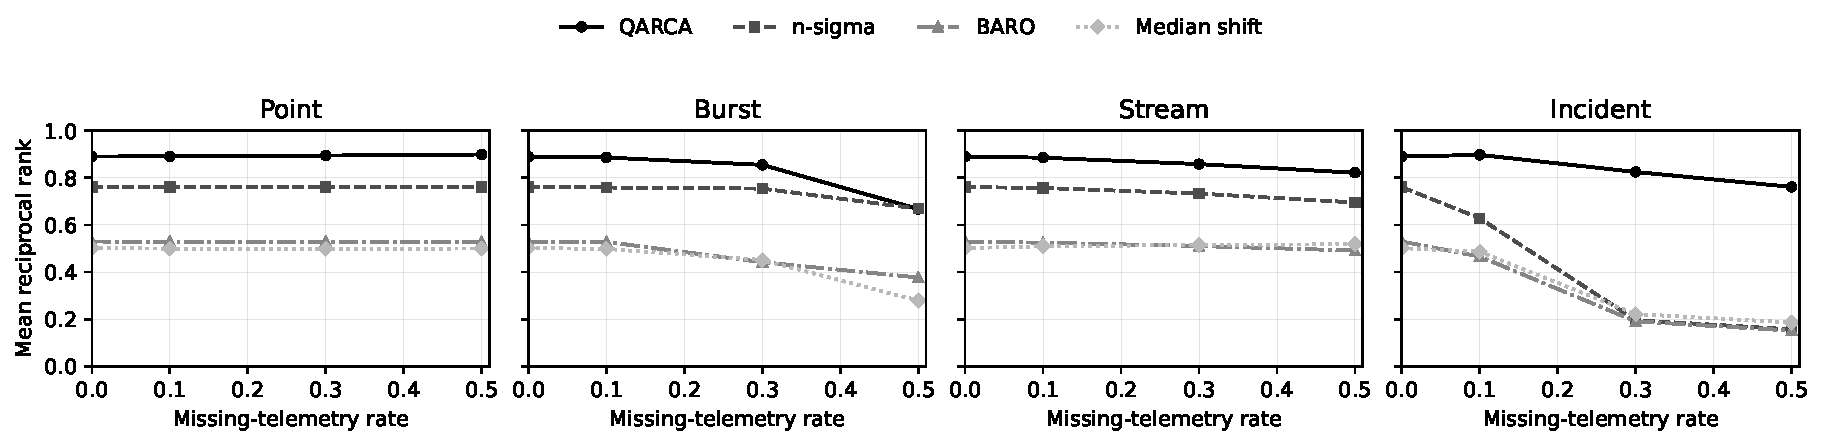
\includegraphics[width=\textwidth]{figures/robustness.pdf}
  \caption{Mean service-level reciprocal rank by loss mechanism and nominal
  rate. Points average masks within each original incident before aggregation;
  complete uncertainty and paired comparisons are reported in the generated
  tables.}
  \label{fig:robustness}
  \Description{Four grayscale line-chart panels show mean reciprocal rank from
  zero to 50 percent added missing telemetry for point, channel-local burst, stream, and
  incident-correlated loss. One line represents each method; distinct marker
  shapes and line styles distinguish methods without relying on color. Exact
  values and trends are listed in figures/alt-text.txt and the result tables.}
\end{figure}
}{%
  \pendingresults{The robustness figure and its plain-text alternative
  description will be generated together after the confirmatory run.}
}

\IfFileExists{generated/results_summary.tex}{%
  % Generated; do not edit.
After averaging masks within each incident, QARCA obtained an original-telemetry MRR of 0.890 and a four-mechanism mean MRR AUC of 0.857. The strongest baseline by the same AUC was $n$-sigma at 0.653; QARCA was 0.204 higher. Within the pre-specified family of 12 paired sign-flip comparisons, 12 favored QARCA and 0 favored a baseline at Holm-adjusted $p<0.05$.

}{%
  \pendingresults{Insert generated per-mechanism robustness AUCs, paired
  QARCA--baseline differences with 95\% intervals, Holm-adjusted tests, and
  mechanism-specific interpretation. The narrative must not be written before
  the result file exists.}
}

\subsection{Ambiguity, ablations, and cost (RQ3--RQ4)}

\IfFileExists{generated/ablation_summary.tex}{%
  % Generated by scripts/analyze_results.py; do not edit.
\begin{table}[t]
\caption{Pre-specified QARCA ablations and diagnostics. Delta is relative to QARCA; higher MRR and AUC are better.}
\label{tab:ablation}
\centering\small
\begin{tabular}{lrrr}
\hline
Variant & Original MRR & MRR AUC & $\Delta$ AUC \\
\hline
QARCA & 0.890 & 0.857 & +0.000 \\
QARCA (original-only train) & 0.862 & 0.665 & -0.192 \\
QARCA (no quality) & 0.897 & 0.782 & -0.075 \\
No quality, original-only train & 0.869 & 0.749 & -0.108 \\
Structural only & 0.230 & 0.230 & -0.627 \\
Quality only & 0.271 & 0.389 & -0.467 \\
No incident-loss train & 0.892 & 0.788 & -0.068 \\
\hline
\end{tabular}
\end{table}

Before imposed loss, the mean native missing-value fraction was 0.3%; all synthetic masks were applied only to originally finite values.
At 50% imposed loss, averaged across mechanisms, 99.7% of QARCA masks retained at least one diagnostically scorable root stream. Its unconditional MRR was 0.787, versus 0.789 when summarized only over incidents with retained root evidence; the unconditional value remains the primary result.
At the same loss endpoint, the label-free top-two margin yielded mean Hit@1 error 0.243 at 50.1% empirical coverage, compared with 0.319 at full coverage. This post-hoc risk--coverage description does not validate a deployment threshold.
Recorded QARCA inference averaged 901.4 ms per incident-condition, while fitting a held-out-system fold averaged 5.3 s; these implementation- and hardware-specific timings are descriptive.

}{%
  \pendingresults{Report unconditional versus root-evidence-conditional
  metrics, risk--coverage characterization, the complete 2-by-2 ablations,
  diagnostic controls, and training/inference runtime. Distinguish descriptive
  fault/system patterns from confirmatory comparisons.}
}

\section{Discussion}

\subsection{How the eventual result should be interpreted}

The design supports a claim about relative service-localization robustness on
the RE1 metric benchmark, not a universal claim about production RCA. If QARCA
improves matched robustness AUC, the defensible interpretation is that explicit
evidence-quality summaries and corruption augmentation help a simple ranker
transfer across these three systems. It would not establish that logistic
ranking is preferable to topology-, trace-, log-, or language-model-based RCA
when those methods receive their required modalities. Conversely, failure to
improve would be informative: missingness indicators may not compensate for
lost causal evidence, or cross-system feature relations may be unstable.

Mechanism-specific outcomes matter more than one average loss rate. Similar
performance under point loss but a drop under stream loss would indicate that
interpolation is not the central challenge; the problem is the removal of an
entire diagnostic channel. Incident-correlated deletion is intentionally
adversarial to anomaly evidence. It should be read as a sensitivity analysis
for MNAR telemetry, not an estimate of how often a production pipeline deletes
high-deviation values.

Root-evidence conditioning is also diagnostic rather than a replacement for
unconditional reporting. Excluding cases with no root stream would inflate the
headline score, so unconditional MRR remains primary. Conditional summaries
answer a different engineering question: how well does the ranker use evidence
when at least some root-service telemetry survives? The gap between the two can
motivate observability redundancy or an abstention policy, but this experiment
does not validate the human and operational cost of abstention.

\subsection{Threats to validity}

\paragraph{Construct validity.}
The injected component is used as the benchmark's localization target. A real
incident can have multiple interacting technical causes and organizational
contributors, so ``root cause'' should not be read as unique causality. The
known injection boundary removes detector error, and the metric-only RE1 subset
does not test cross-modal alignment. MRR rewards early placement but does not
measure explanation quality or time-to-repair; the secondary metrics expose
some, not all, alternatives.

\paragraph{Internal validity.}
Synthetic deletion preserves the recorded values outside the mask and cannot
recreate feedback between application failure and telemetry infrastructure.
The incident-correlated mechanism uses a particular exponential weighting;
other MNAR processes may differ. Deterministic seeds and matched masks reduce
random comparison noise but do not remove model misspecification. Causal fill
can favor persistent signals and suppress short anomalies, whereas QARCA sees
the mask explicitly. This is part of the estimand---robustness of the complete
method pipeline---but should not be mistaken for a pure comparison of scoring
functions.

Folder structure contains service and fault labels. Tests verify that changing
case, system, root, or fault metadata does not change extracted features, and
the estimator receives only the fixed numeric columns. Nevertheless, metric
composition can reveal coarse system structure. LOSO evaluation is therefore
necessary but cannot prove absence of every indirect system cue. Training-mask
namespaces, fixed folds, and per-incident weighting limit leakage; release of
per-case predictions permits independent audit.

\paragraph{External validity.}
Online Boutique, Sock Shop, and Train Ticket are widely used open-source or
demonstration systems, not a representative sample of industrial architectures,
traffic patterns, or observability stacks. RE1 contains a balanced grid of five
services, five fault types, and five repetitions per system, unlike production
fault prevalence. The study should be replicated on naturally incomplete
telemetry and on systems where topology and service identities evolve.

\paragraph{Conclusion validity.}
Masks within an incident are correlated, which is why inference aggregates
them before paired testing. Three held-out systems remain too few for a
population-level claim about systems; incident-level intervals quantify
variation in this benchmark only. Multiple primary comparisons are corrected,
while uncorrected fault and system slices are labeled descriptive. A protocol
deviation, incomplete run, or mismatch between saved predictions and generated
tables invalidates confirmatory wording and must be reported.

\section{Reproducibility and Artifact Statement}

The working artifact pins Python 3.12 and exact versions of NumPy, pandas,
SciPy, scikit-learn, Matplotlib, and \texttt{fse-baro}. It includes the data
manifest and archive checksums, deterministic corruption code, feature and
leakage tests, LOSO runners, raw per-case prediction schema, aggregation,
paired inference, figures, and alternative text. RCAEval archives are obtained
separately from the dataset DOI and are not redistributed. A reviewer-facing
artifact must exclude author-identifying repository history while preserving
the exact source used to generate the submitted PDF.

At review time, the anonymous artifact location is
\texttt{\artifactlocation}. \textbf{This placeholder must be replaced and tested
from a clean environment before submission.} The final release license, frozen
revision identifier, and archival DOI require author confirmation. Reproduction
starts from the documented archive hashes, executes unit tests, runs the frozen
experiment, and regenerates all manuscript result inputs; handwritten numerical
claims are not part of that path.

\section{Conclusion}

This work frames incomplete observability as part of microservice diagnosis
rather than a preprocessing nuisance. It defines matched structured loss on
RCAEval RE1 and a leakage-conscious LOSO evaluation of QARCA against three
metric baselines. The protocol distinguishes point, channel-local burst, stream, and
incident-correlated loss; preserves missingness as evidence; and treats masks
as repeated measures.
\IfFileExists{generated/conclusion_result.tex}{%
  % Generated; do not edit.
Under the evaluated synthetic metric-loss masks, QARCA's mean MRR AUC was 0.857 versus 0.653 for the strongest baseline (+0.204); 12 of 12 Holm-adjusted comparisons favored QARCA. These results do not establish performance under naturally occurring telemetry outages or telemetry modalities absent from RCAEval RE1.
%
}{%
  \textbf{A performance conclusion will be added only after the confirmatory
  result files are generated and audited.}%
}

\typeout{BODY-END-PAGE=\thepage}

\section*{Acknowledgements and Use of AI-Assisted Tools}

For manuscript preparation, OpenAI Codex was used on 22 July 2026 to assist
with literature organization, experimental-software scaffolding, and initial
language drafting. The system is not an author. Before submission, the human
authors must run and inspect the complete experiment, verify every citation and
numerical statement against its primary source or saved output, revise the text
where necessary, approve the final manuscript, and accept full responsibility
for its content. Funding and non-author acknowledgements are withheld from this
anonymous working version and require author-supplied text for camera-ready
publication.

\section*{Disclosure of Interests}

\ifanonymous
The authors' declaration has not yet been provided to the drafting system. A
complete author-confirmed disclosure must replace this sentence before
submission or be supplied in the venue-approved anonymous form. This statement
must not be interpreted as a declaration that no competing interests exist.
\else
\intereststatement
\fi

\bibliographystyle{splncs04}
\bibliography{references}

\end{document}
